Sentiment analysis, also known as opinion mining, aims to determine the sentiment or subjective information expressed in a piece of text. It involves analyzing text data to identify the overall sentiment, such as positive, negative, or neutral, and sometimes even more nuanced emotions. One popular model used in sentiment analysis is the \ac{vad} model~\cite{VAD-MODEL}.

\subsubsection{\acs{vad} Sentiment Model}

The traditional \acs{vad} model assigns scores to words based upon three dimensions: valence, arousal, and dominance. Valence represents the pleasantness or positivity of the sentiment, arousal represents the level of excitement or intensity, and dominance represents the degree of control or influence.

\begin{figure}[Valence-Arousal-Dominance sentiment models]{FIG:SentimentModels}{Sentiment models based on valence, arousal \& dominance, left representing the Valence-Arousal model~\cite{WIKI:VA-MODEL}, right representing the \acl{vad} model~\cite{WIKI:PAD-MODEL}.}
    \begin{subfigure}[SBFIG:VAModel]{Circumplex Valence-Arousal model}{\includesvg[inkscapelatex=false,width=0.42\textwidth]{VAModel}}
    \end{subfigure}
    \begin{subfigure}[SBFIG:VADModel]{Three-dimensional \acl{vad} model}{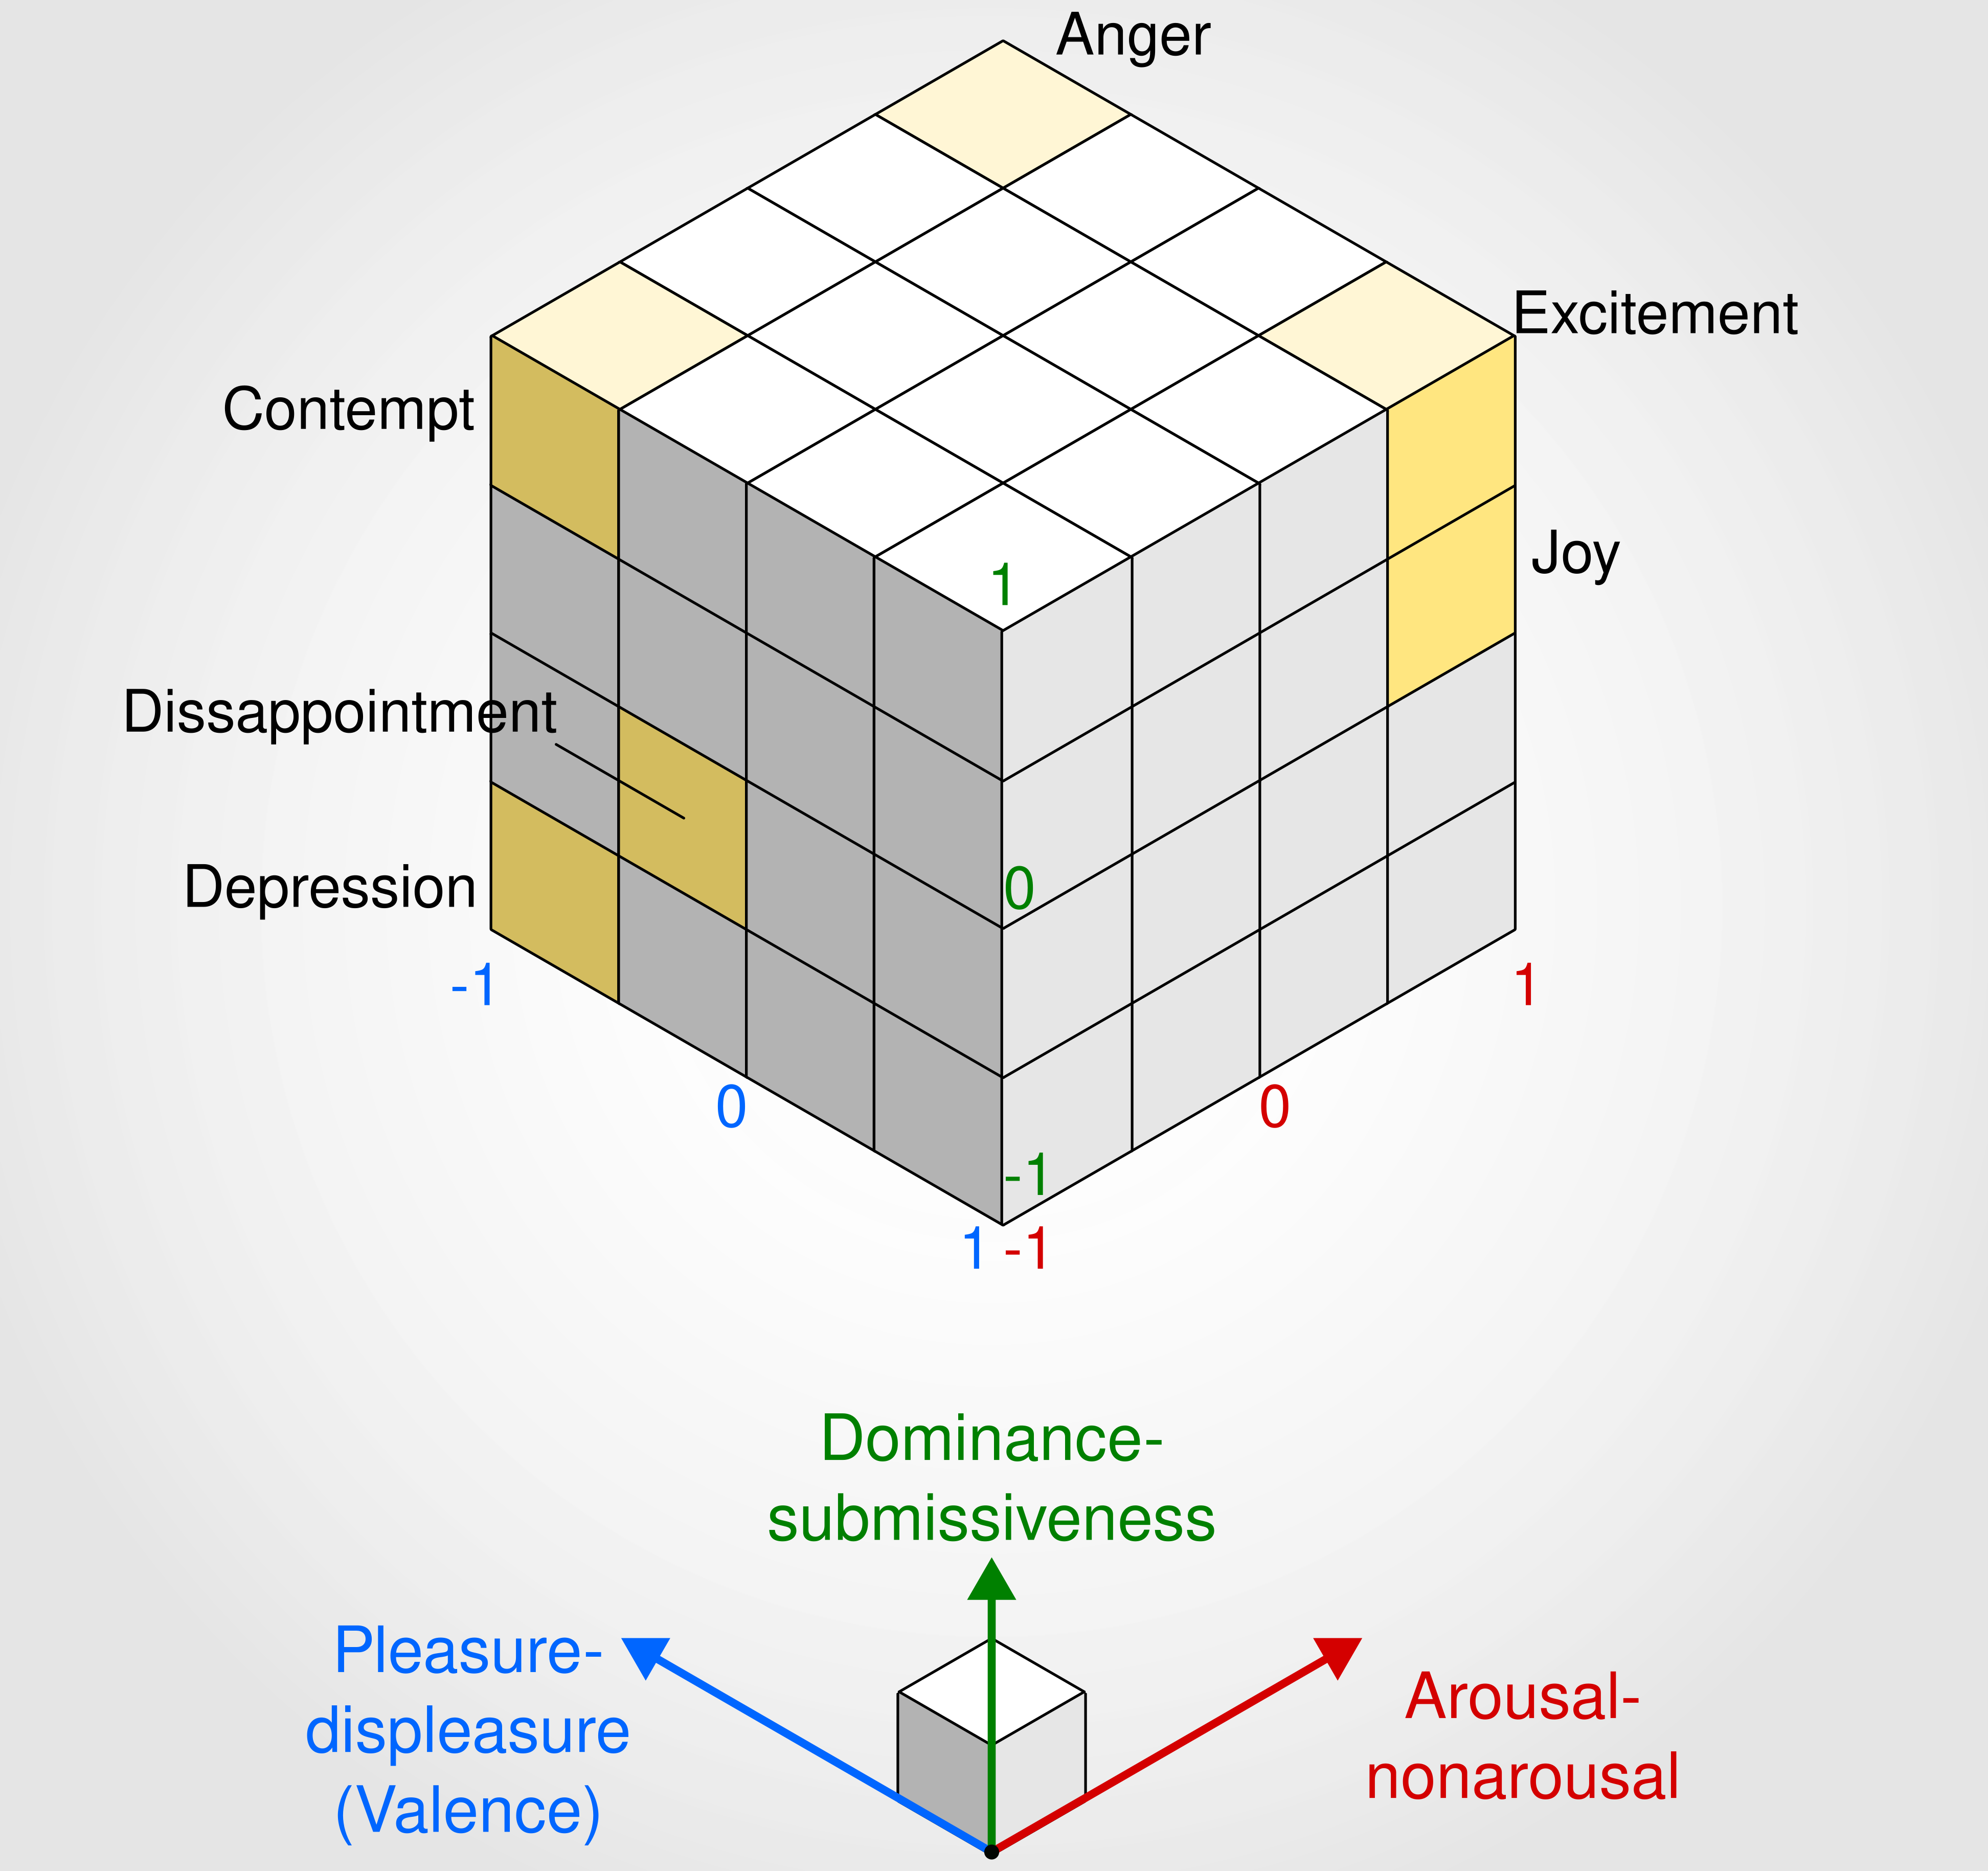
\includegraphics[width=0.445\textwidth]{img/VADModel.png}}
    \end{subfigure}
\end{figure}

Frequently, valence and arousal have been considered sufficiently independent to convey mood and musical emotions [\ref{SBFIG:VAModel}], since two dimensions are enough to represent a reliable sentiment spectrum, striking a balance between complexity and predictive potential; with dominance being necessary for a wider range of emotions [\ref{SBFIG:VADModel}], at the expense of simplicity and scoring accuracy. These scores provide a more comprehensive understanding of the emotions conveyed in the text~\cite{EMOTION-MODELS}.

\subsubsection{Sentiment Ratio}

Another common approach in sentiment analysis is to calculate a sentiment score from the frequency of positive and negative words in the text [\ref{EQ:StRatio}]. This score can be computed by subtracting the number of negative words from the number of positive words and dividing it by the total number of words in the text. This technique provides a sentiment ratio, a quantitative measure of sentiment polarity that is akin to valence but ignoring neutral words~\cite{STSC}.

\begin{equation}[EQ:StRatio]{Sentiment Ratio}
    Sentiment\;Ratio = \frac{|Positive\;words| - |Negative\;words|}{|Total\;words|} \in [-1, 1]
\end{equation}